\documentclass{article}

% We suggest
% if you need to pass options to natbib, use, e.g.:
%     \PassOptionsToPackage{numbers, compress}{natbib}
% before loading neurips_2020

% ready for submission
% \usepackage{neurips_2020}

% to compile a preprint version, e.g., for submission to arXiv, add add the
% [preprint] option:
%     \usepackage[preprint]{neurips_2020_tda}

% to compile a camera-ready version, add the [final] option, e.g.:
%\usepackage[final,nonatbib]{neurips_2020_tda}

% to avoid loading the natbib package, add option nonatbib:
\usepackage[nonatbib]{neurips_2020_tda}

\usepackage[utf8]{inputenc} % allow utf-8 input
\usepackage[T1]{fontenc}    % use 8-bit T1 fonts
\usepackage{amsfonts}       % blackboard math symbols
\usepackage{booktabs}       % professional-quality tables
\usepackage{hyperref}       % hyperlinks
\usepackage{url}            % simple URL typesetting
\usepackage{microtype}      % microtypography
\usepackage{nicefrac}       % compact symbols for 1/2, etc.
\usepackage{paralist}       % in-paragraph enumerations
\usepackage{siunitx}        % SI units
%%For figures and subcaptions
\usepackage[font=small]{caption}
\usepackage[labelformat=empty, position=top]{subcaption}
\usepackage{subcaption}
\usepackage[export]{adjustbox}

\usepackage{amsmath,amssymb,amsfonts,amsthm}
\usepackage{microtype}
%\usepackage[draft]{fixme}
\usepackage{algorithmic}
\usepackage{graphicx}
\usepackage{textcomp}
\usepackage{xcolor}
\usepackage{tikz}
\usepackage{mwe}
\usepackage{blkarray}

\usepackage{dcolumn,booktabs}
\newcolumntype{d}[1]{D{.}{.}{#1}}
\newcommand\mc[1]{\multicolumn{1}{c}{#1}} % handy shortcut macro

\newsavebox{\tempbox}
\newlength{\tempwidth}


\usepackage[natbib,hyperref,sorting=none]{biblatex}
%\usepackage[backend=bibtex,doi=true,style=numeric,maxnames=3,maxbibnames=6]{biblatex}
\addbibresource{bibliography.bib}
%\renewcommand*{\bibfont}{\footnotesize}

\urlstyle{same}

\title{
  Simplicial Neural Networks
}

% The \author macro works with any number of authors. There are two commands
% used to separate the names and addresses of multiple authors: \And and \AND.
%
% Using \And between authors leaves it to LaTeX to determine where to break the
% lines. Using \AND forces a line break at that point. So, if LaTeX puts 3 of 4
% authors names on the first line, and the last on the second line, try using
% \AND instead of \And before the third author name.

\author{%
  Stefania Ebli \\
  Laboratory for Topology and Neuroscience\\
  EPFL, Lausanne, Switzerland\\
  \texttt{stefania.ebli@epfl.ch}\\
  % examples of more authors
  \And
  Gard Spreemann\thanks{Work done while at the EPFL. Present affiliation: Telenor Research, Fornebu, Norway.} \\
  Laboratory for Topology and Neuroscience\\
  EPFL, Lausanne, Switzerland\\
  \texttt{gspr@nonempty.org} \\
  \And
  Michaël Defferrard \\
  EPFL, Lausanne, Switzerland\\
  \texttt{michael.defferrard@epfl.ch} 
  % \And
  % Coauthor \\
  % Affiliation \\
  % Address \\
  % \texttt{email} \\
  % \And
  % Coauthor \\
  % Affiliation \\
  % Address \\
  % \texttt{email} \\
}
\theoremstyle{definition}
\newtheorem{definition}{Definition}
\newtheorem{example}[definition]{Example}
\newtheorem{note}[definition]{Note}

\theoremstyle{plain}
\newtheorem{theorem}[definition]{Theorem}
\newtheorem{lemma}[definition]{Lemma}
\newtheorem{proposition}[definition]{Proposition}
\newtheorem{corollary}[definition]{Corollary}

\definecolor{mplC0}{HTML}{1f77b4}
\definecolor{mplC1}{HTML}{ff7f0e}
\definecolor{mplC2}{HTML}{2ca02c}
\definecolor{mplC3}{HTML}{d62728}
\definecolor{mplC4}{HTML}{9467bd}
\definecolor{mplC5}{HTML}{8c564b}
\definecolor{mplC6}{HTML}{e377c2}
\definecolor{mplC7}{HTML}{7f7f7f}
\definecolor{mplC8}{HTML}{bcbd22}
\definecolor{mplC9}{HTML}{17becf}

\newcommand{\RR}{\ensuremath{\mathbb{R}}}
\newcommand{\ZZ}{\ensuremath{\mathbb{Z}}}
\newcommand{\RP}{\ensuremath{\mathbb{RP}}}
\newcommand{\lapu}{\ensuremath{\mathcal{L}^{\text{up}}}}
\newcommand{\lapd}{\ensuremath{\mathcal{L}^{\text{down}}}}
\newcommand{\lap}{\ensuremath{\mathcal{L}}}
\newcommand{\iso}{\ensuremath{\cong}}
\newcommand{\rank}{\ensuremath{\text{rank}}}
\newcommand{\inv}{\ensuremath{^{-1}}}
\newcommand{\transpose}{\ensuremath{^{\intercal}}}


\newcommand{\ie}{}
\def\ie/{i.e.}
\newcommand{\eg}{}
\def\eg/{e.g.}
\newcommand{\etc}{}
\def\etc/{etc.}

\newcommand{\gardfix}[2]{{\color{red}#1}\fxfatal{#2}}
\newcommand{\fix}[2]{{\color{red}#1}\fxfatal{#2}}
\newcommand{\thmcite}[1]{\citeauthor{#1}, \citeyear{#1}~\cite{#1}}
\newcommand{\suchthat}{\ensuremath{\, \mid \,}}

\newcommand{\Reffig}[1]{Figure~\ref{fig:#1}}
\newcommand{\reffig}[1]{figure~\ref{fig:#1}}
\newcommand{\refeq}[1]{equation~\eqref{eq:#1}}
\newcommand{\refsec}[1]{section~\ref{sec:#1}}

\newcommand{\ip}[2]{\ensuremath{\left\langle #1 , #2 \right\rangle}}
\newcommand{\norm}[1]{\ensuremath{\lVert #1 \rVert}}

\newcommand{\placeholderfigure}{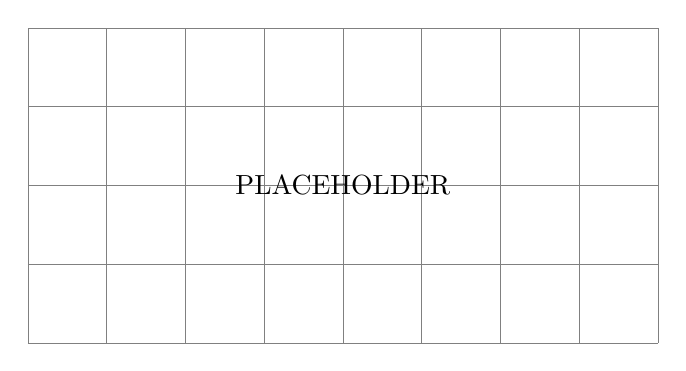
\begin{tikzpicture}
      \draw[help lines] (0, 0) grid (8, 4);
      \node () at (4,2) {PLACEHOLDER};
  \end{tikzpicture}
}

\DeclareMathOperator{\cut}{cut}
\DeclareMathOperator{\im}{im}
\DeclareMathOperator{\proj}{proj}
\DeclareMathOperator{\VR}{VR}
\DeclareMathOperator{\diag}{diag}


%---------For commenting--------
\usepackage{color}
\definecolor{darkorchid}{rgb}{0.6,0.196,0.8}
\newcommand{\todo}[1]{{\color{red}[[\textbf{TODO: }#1]]}}
\newcommand{\stefania}[1]{{\color{mplC0}[[\textbf{Stefania says: }#1]]}}
\newcommand{\gard}[1]{{\color{mplC2}[[\textbf{Gard says: }#1]]}}
\newcommand{\mdeff}[1]{{\color{mplC1}[[\textbf{Michaël says: }#1]]}}

%--------For Referencing--------
\newcommand{\appendref}[1]{Section~\ref{append:#1}}
\newcommand{\figref}[1]{Figure~\ref{fig:#1}}
\newcommand{\exref}[1]{Example~\ref{ex:#1}}
\newcommand{\secref}[1]{Section~\ref{sec:#1}}
\newcommand{\Thmref}[1]{Theorem~\ref{thm:#1}}
\newcommand{\thmref}[1]{Theorem~\ref{thm:#1}}
\newcommand{\defref}[1]{Definition~\ref{def:#1}}


\begin{document}

\maketitle

\begin{abstract}
In this paper we present simplicial neural networks (SNNs)\gard{I feel the word convolution should be in the name. There can potentially be other simplicial networks out there; ours are decidedly \emph{convolutional}.} \stefania{ASked also K about the title. THere are no simplicial neural networks out there. Even if simplicial convolutional neural networks is maybe a more complete name we think simplicial neutal networks is more catchy..}, a generalization of graph convolutional neural networks to data that live on a class of topological spaces called simplicial complexes. These are natural multi-dimensional extensions of graphs which encode more than just pairwise relationships, namely higher-order relationships between nodes (represented geometrically as filled triangles, tetrahedra, and so forth). We define an appropriate notion of convolutions for such data, which we leverage to construct the desired convolutional neural networks. This allows us to consider richer data than traditional methods, including $n$-fold collaboration networks and vector field data.
  
\end{abstract}


\section{Introduction}

Graph-based convolutional neural networks (GNNs) have recently become popular techniques in machine learning~\cite{defferrard2016convolutional, bronstein2017geometric, wu2020survey}. Compared to classical convolutional deep neural networks that work with regular grid-structured data, graph neural networks can take into account irregular graphs to better learn complex interactions in the data~\cite{battaglia2018relational}. Although graphs are useful in describing complex systems of irregular relations in a variety of settings, they are intrinsically limited to modeling pairwise relationships. The advance of topological methods in machine learning~\cite{Gabrielsson2020topological, Hofer2019LearningRO, rieck2018neural}, and the earlier establishment of \emph{topological data analysis (TDA)}~\cite{carlsson2008,chazal2017,edelsbrunner2010computational,ghrist2008barcodes} as a field in its own right, have confirmed the usefulness of viewing data as topological spaces in general, or in particular as simplicial complexes, which can be thought of as a higher-dimensional analog of graphs~\cite{moore2012,patania2017}.

We here take the view that structure is encoded in \emph{simplicial complexes}, and that these represent $n$-fold interactions between objects. In this setting, we present \emph{simplicial neural networks (SNNs)}, a novel neural network framework that take into account locality of data living over a simplicial complex in the same way a GNN does for graphs or a conventional convolutional network does for grids. We show some useful properties of SNNs, indicate how they can be implemented as sparse matrix multiplications, and finally demonstrate the efficacy of the network on a dataset built from coauthorship data.

Other approaches, such as hypergraph neural networks~\cite{feng2018hypergraphs}, do not have connections to the global topological structure of the simplicial complex, a highly relevant aspect in TDA. This leads us to believe that our method is far better suited for situations where that is relevant, such as perhaps in the processing of data that exists naturally as vector fields or data that is sensitive to the space's global structure~\cite{perraudin2019deepsphere}.


\section{Proposed Method}

In this section we review the notion of a simplicial complex and its associated Laplacians, before we introduce the simplicial neural networks. 

%\subsection{Simplicial Complexes}
\textbf{Simplicial Complexes.} A \emph{simplicial complex} is a collection of finite sets closed under taking subsets. We call a member of a simplicial complex $K$ a \emph{simplex} of \emph{dimension $p$} if it has cardinality $p+1$, and denote the set of all such $K_p$. A $p$-simplex has $p+1$ \emph{faces} of dimension $p-1$, namely the subsets omitting one element. We denote these $[v_0,\dotsc,\hat{v}_i,\dotsc, v_p]$ when omitting the $i$'th element. If a simplex $\sigma$ is a face of $\tau$, we say that $\tau$ is a \emph{coface} is $\sigma$. While this definition is entirely combinatorial, there is a geometric interpretation, and it will make sense to refer to and think of $0$-simplices as \emph{vertices}, $1$-simplices as \emph{edges}, $2$-simplices as \emph{triangles}, $3$-simplices as \emph{tetrahedra}, and so forth (see Figure~\ref{fig:data2complex}, (b)).

Let $C^p(K)$ be the set of functions $K_p\to\RR$, with the obvious vector space structure. These \emph{$p$-cochains} will encode our data. Define the linear \emph{coboundary} maps $\delta^p:C^p(K)\to C^{p+1}(K)$ by
\begin{equation*}
\delta^p(f)([v_0,\dotsc,v_{p+1}]) = \sum_{i=0}^{p+1} (-1)^i f([v_0,\dotsc,\hat{v}_i,\dotsc,v_{p+1}]).
\end{equation*}

\begin{figure}[htpb]
%\begin{table*}[!t]
\savebox{\tempbox}{% compute size of tabulat
\scriptsize{
\begin{tabular}{llll}
    \cmidrule(r){1-3}
    Papers   & Authors     & Citations  \\
    \midrule
    Paper I & A, B, C  & 100  \\
    Paper II &  A, B & 50\\ 
    Paper III & A, D & 10\\ 
    Paper IV & C, D & 4\\ 
    \bottomrule
  \end{tabular}
}}%
\settowidth{\tempwidth}{\usebox{\tempbox}}%
\hfil\begin{minipage}[b]{\tempwidth}%
\raisebox{-\height}{\usebox{\tempbox}}%
%\vspace{-7pt}
\scriptsize{\caption*{(a)}}%
\label{table:data}%
\end{minipage}%
\savebox{\tempbox}{\includegraphics[height=2.3cm]{./figures/cc1.png}}%
\settowidth{\tempwidth}{\usebox{\tempbox}}%
\hfil\begin{minipage}[b]{\tempwidth}%
\raisebox{-\height}{\usebox{\tempbox}}%
\scriptsize{\captionof*{figure}{(b)}}%
\label{fig:co-authoship-complex}%
\end{minipage}%
\vspace{5pt}
%\end{table*}
\savebox{\tempbox}{\scriptsize{
\begin{blockarray}{cccccc}
\tiny{AB} & \tiny{AC} & \tiny{AD} & \tiny{BC} & \tiny{CD} \\
\begin{block}{(ccccc)c}
  3 & 0 & 1 & 0 & 0 & \tiny{AB} \\
  0 & 3 & 1 & 0 & -1 & \tiny{AC} \\
  1 & 1 & 2 & 0 & 1 & \tiny{AD} \\
  0 & 0 & 0 & 3 & -1 & \tiny{BC}\\
  0 & -1 & 1 & -1 & 2 & \tiny{CD}\\
\end{block}
\end{blockarray}}}%
\settowidth{\tempwidth}{\usebox{\tempbox}}%
\hfil\begin{minipage}[b]{\tempwidth}%
\raisebox{-\height}{\usebox{\tempbox}}%
\scriptsize{\captionof*{figure}{(c)}}%
\end{minipage}%
%\end{table*}
\caption{Example of co-authorship complex and its $1$-Laplacian. (a) Data. (b) Co-authorship complex with corresponding cochains build from the data. (c) $1$-Laplacian associated to the co-authorship complex. }\label{fig:data2complex}
\end{figure}

%\subsection{Simplicial Laplacians}
\textbf{Simplicial Laplacians.} We are in this paper concerned with finite abstract simplicial complexes, although our method is applicable to a much broader setting, such as for example finite CW-complexes. %\gard{I kinda liked the point that emphasized that the simplicial complexes don't need an embedding, but maybe there isn't space for it?}
%In particular, it is not necessary for the simplicial complexes to come equipped with some embedding into Euclidean spaces, nor do we demand that they triangulate a Riemannian manifold.
In analogy with Hodge--de Rham theory~\cite{madsen1997calculus}, we then define the \emph{degree-$i$ simplicial Laplacian} of a simplicial complex $K$ as the linear map $\lap_i:C^i(K)\to C^i(K)$ specified by
\begin{equation*}
  \lap_i = \lapu_i + \lapd_i = \delta^{{i}^{\ast}}\circ\delta^{i} + \delta^{i-1}\circ\delta^{{i-1}^{\ast}},
\end{equation*}

where $\delta^{{i}^{\ast}}$ is the adjoint of the coboundary with respect to the inner product (for example the one making the indicator function basis orthonormal). In the case $i=0$, $\mathcal{L}_0$ is the classical graph Laplacian. In most practical applications, the coboundary can be represented as a sparse matrix $B_i$ and the Laplacians can be efficiently computed as $L_i=B_i^T B_{i}+B_{i-1}B_{i-1}^T$. \stefania{Still thinking about moving this to the appendix} Since the Laplacians encode information about the adjacency of the simplices, they can be interpreted as a message passing functions~\cite{gilmer2017NeuralMP}. Additionally, they carry valuable topological information about the simplicial complex. In particular, the kernel of the $k$-Laplacian is isomorphic to the $k$-(co)homology of its associated simplicial complex~\cite{eckmann1944,horak2013spectra}.
% In other words, the number of zero-eigenvalues tells us the number of $k$-dimensional holes~\cite{horak2013spectra}.


\paragraph{Simplicial convolution.}

A convolutional layer is of the form $f\ast \varphi_W$, where $\ast$ denotes convolution, and $\varphi_W$ is a function
\emph{with small support} parameterized by learnable weights $W$.
Typically, $\varphi_W$ is locally constant in a small spatial region, and is zero elsewhere. This formulation of CNNs lends itself to a spectral interpretation that we exploit to extend CNNs to a much more general setting.

Following~\cite{defferrard2016convolutional} and motivated by the fact that the discrete Fourier transform of a real-valued function on an $n$-dimensional cubical grid coincides with its decomposition into a linear combination of the eigenfunctions of the graph Laplacian for that grid, we define the Fourier transform $\mathcal{F}_p: C^p(K) \to \mathbb{R}^{\lvert K_p \rvert}$ of real $p$-cochains on a simplicial complex with Laplacians $\mathcal{L}_p$ as $\mathcal{F}_p(c) = \left(\ip{c}{e_1}_p, \ip{c}{e_2}_p, \dotsc, \ip{c}{e_{\lvert K_p \rvert}}_p\right)$, where the $e_i$'s are the eigencochains of $\mathcal{L}_p$ ordered by eigenvalues $\lambda_1\leq\dotsm\leq\lambda_{\lvert K_p \rvert}$. The function $\mathcal{F}_p$ is invertible since $\mathcal{L}_p$ is diagonalizable; explicitly, if we write $U\diag(\Lambda)U\transpose$ for a normalized eigendecomposition, the orthonormal matrices $U$ and $U\transpose$ represent $\mathcal{F}\inv_p$ and $\mathcal{F}_p$, respectively. This is the foundation for Barbarossa's development of signal processing on simplicial complexes~\cite{barbarossa2018learning}.

Recall that on the function classes for which it is defined, the classical Fourier transform satisfies $\mathcal{F}(f\ast g)=\mathcal{F}(f)\mathcal{F}(g)$, where the right-hand side denotes pointwise multiplication. This will be our definition of convolution in the simplicial setting. Indeed, for cochains $c,c'\in C^p(K)$ we \emph{define} their convolution as the cochain $c\ast_p c' = \mathcal{F}_p\inv\left(\mathcal{F}_p(c)\mathcal{F}_p(c')\right)$.

Within this framework, we are led to define a \emph{simplicial convolutional layer} with input $p$-cochain $c$ and weights $W$ as being of the form $\mathcal{F}\inv_p(\varphi_W)\ast_p c$ for some as of yet unspecified $\varphi_W\in\mathbb{R}^{\lvert K_p \rvert}$. To ensure the central property that a convolutional layer be localizing, we demand that $\varphi_W$ be a low-degree polynomial in $\Lambda=(\lambda_1, \dotsc, \lambda_{\lvert K_p \rvert})$, namely
\begin{equation*}
  \varphi_W = \sum_{i=0}^N W_i\Lambda^i = \sum_{i=0}^N W_i(\lambda^i_1, \lambda^i_2, \dotsc, \lambda^i_{\lvert K_p \rvert}),
\end{equation*}
for small $N$. In signal processing parlance, one would say that such a convolutional layer \emph{learns filters that are low-degree polynomials in the frequency domain}.

The reason for restricting the filters to be these low-degree polynomials is best appreciated when writing out the convolutional layer in a basis. Let $L^i_p$ denote the $i$'th power of the matrix for $\mathcal{L}_p$ in, say, the standard basis for $C^p(K)$, and similarly for $c$. Then
\begin{equation*}
  \mathcal{F}\inv_p(\varphi_W)\ast_p c = \sum_{i=0}^N W_iU\diag(\Lambda^i)U\transpose c = \sum_{i=0}^N W_i\left(U\diag(\Lambda)U\transpose\right)^i c = \sum_{i=0}^NW_iL^i_pc. %\label{eq:filter}
\end{equation*}
This is important for three reasons, like for traditional CNNs.
First, the convolution can be efficiently implemented by $N$ sparse matrix-vector multiplications: This reduces the computational complexity from $\mathcal{O}(\lvert K_p\rvert^2)$ to $\mathcal{O}(\xi\lvert K_p\rvert)$ where $\xi$ is the density factor.
Second, the number of weights to be learned is reduced from $\mathcal{O}(\lvert K_p\rvert)$ to $\mathcal{O}(1)$.
Third, the operation is $N$-localizing in the sense that if two simplices $\sigma,\tau$ are more than $N$ hops apart, then a degree-$N$ convolutional layer does not cause interaction between $c(\sigma)$ and $c(\tau)$ in its output (see the supplementary material).
Those local interactions (in the spatial domain) can be interpreted as message-passing between simplices~\cite{gilmer2017NeuralMP}.

%In practice we implement \refeq{filter} using Chebyshev polynomials, as suggested for GNNs in~\cite{defferrard2016convolutional}.
%\mdeff{Not very important: The choice of polynomial (monomials, Chebyshev, Legendre, etc.) doesn't make much difference in practice.}



\section{Experimental Results}

%\paragraph{Task/Problem.}
As many real-world datasets contain missing values, missing data imputation (MDI) has been a popular problem to tackle in statistics and machine learning~\cite{little1986statistical, nelwamondo2007missing}.
GNNs have recently proved to be a powerful tool for this task~\cite{spinelli2020neural}.
With a view that our method incorporates additional higher-dimensional structure in the data, we evaluate the performance of the SNNs in imputing missing data over simplicial complexes.

\paragraph{Data.}
A \emph{co-authorship complex}~\cite{patania2017} is a simplicial complex where a paper with $k$ authors is represented by a $(k-1)$-simplex.
\mdeff{Projection of the paper-author bipartite graph? Discuss why not hypergraphs? Not sure.}\stefania{Added this in the appendix}
By subset closure, vertices represent authors and the added subsimplices of the $k-1$-simplex are interpreted as collaborations among subgroups of authors. We sampled two co-authorship complexes---CC1 and CC2, see Table~\ref{table:Simplices-coauthor} for statistics---from the Semantic Scholar Open Research Corpus~\cite{ammar18NAACL}, a dataset of over $39$ million research papers with authors and citations.\footnote{Papers with less than $5$ citations and more than $10$ authors were excluded.}
\mdeff{I have a repo with the code to create this dataset. Shall we make it public and link it here?}\stefania{Sure!}
We believe the following procedure extracts representative papers from which one can construct co-authorship complexes: We performed random walks (of length $80$) on the vertices of the graph which correspond to papers, and edges connect papers sharing at least one author. \mdeff{Needs clarification.}\stefania{Is it more clear like this?}
The $k$-cochains are given by the number of shared citations of the given collaboration (see Figure~\ref{fig:data2complex}).
\mdeff{Could be more precise. Though the figure is great and very helpful.}\stefania{I will add something in the appendix. In a longer version this will be definitely clarified here.}

\paragraph{Method.}
We evaluated the performance of the SNNs on the task of imputing missing data on the $k$-cochains (for $k=0,1,2$) of the extracted co-authorship complexes. As in a typical pipeline for this task~\cite{nelwamondo2007missing}, missing data is artificially introduced by replacing a portion of the values with a constant. Specifically, given a fixed co-authorship complex, missing data is introduced at random on the $k$-cochains at $4$ rates: $10\%,  20\%,  30\%$, and $50\%$. The training input is then given by the $k$-cochains on which the random missing data is substituted by the median of the known data (the median is perhaps a reasonable first guess for estimating missing data). We trained an SNN comprising $3$ layers with $30$ convolutional filters of degree $N=5$. We used the $L_1$ norm as the reconstruction loss over the known elements, and the Adam optimizer with a learning rate of $10^{-3}$. The SNN was trained for $1000$ iterations. We then tested the performance of the network on its accuracy in imputing missing data. As a statistical evaluation, we tested the network on different random samples of the damaged portions for the same percentage of missing value.

\paragraph{Results.}
\gard{Note for me to remember to add a punchline somewhere in this section :-)}
Figure~\ref{fig:accuracy-error} (a-b) shows the mean accuracy (MA) and mean absolute error distribution (MAED) \stefania{change we do not take average histogram} (see Section~\ref{sec:supp_material} for definitions) of the SNN in inputing missing citations on CC1. Observe that the distribution of the prediction error accumulates close to zero.

%\begin{figure}[htbp]
%  \centering
%\includegraphics[scale=0.35]{./figures/distribution_cohain_150250.png}
% \caption{Distribution of the citation in CC1 } \label{fig:accuracy}
%\end{figure}
\begin{figure}[tb]
\centering
 \begin{subfigure}[t]{-0.8\textwidth}
 \vspace{-4cm}
    \text{(a)}
  \end{subfigure}
\begin{subfigure}[t]{0.8\textwidth}
\centering
   \includegraphics[scale=0.35]{./figures/accuracy_network1.png}
 %\caption{Accuracy of SNN in predicting missing citations } \label{fig:accuracy}
\end{subfigure}
 \begin{subfigure}[t]{0.8\textwidth}
    \text{(b)}
  \end{subfigure}
\begin{subfigure}[t]{0.8\textwidth}
\centering
\vspace{-0.5cm}
   \includegraphics[scale=0.36]{./figures/Error_dist_start150250_seed6666_notsee40.png}
 % \caption{Distribution of the prediction's error} \label{fig:error}
\end{subfigure}
\caption{(a) Mean Accuracy $\pm$ std over 5 samples of SNN in imputing missing citations on CC1. (b) Mean Absolute Error $\pm$ std over 5 samples of SNN for $40\%$ missing values in CC1. \stefania{Add error on bins.} \mdeff{I don't get (b).} \mdeff{Some space could be claimed from this figure.}}
\label{fig:accuracy-error}
\end{figure}

As a second assessment, we evaluate how accurately an SNN trained on one co-authorship complex can impute missing citations on a different complex. Over the assumption that co-authorship complexes share a similar structure and the same data underlies the generating process of cochains.
Figure~\ref{fig:transfer-learning} shows the MA in predicting missing citations on CC1 using the above architecture of SNN trained on CC2.
\mdeff{Conclusion? Trained SNN transfer because not much MA is lost, or the hypothesis is satisfied?}

Table~\ref{table:comparison-SNN} shows the performance of three statistical baselines: missing values inferred as the mean or median of all known values, and missing values inferred from the $(k-1)$ and $(k+1)$ neighbors of the simplices ($k$-simplicial neighbor $k$-sn).
\mdeff{Mean or median of the neighbors?}
SNNs well outperform these baselines.
Comparison with other state-of-the-art imputation algorithms is left for future work.

\begin{figure}[htbp]
  \centering
\includegraphics[scale=0.35]{./figures/accuracy_network1_pretrained.png}
  \caption{Mean Accuracy $\pm$ std over 5 samples in imputing missing citations on CC1 with an SNN trained on CC2.} \label{fig:transfer-learning}
\end{figure}

%\scriptsize{
\begin{table}[htbp]
  \centering
  \scriptsize{
  \begin{tabular}{lcccccc}
    \toprule
    Method   & CC1 - dim 0   & CC1 - dim 1   & CC1 - dim 2   & CC2 - dim 0  & CC2 - dim 1  & CC2 - dim 2 \\
    \midrule
    Mean & $3.3 \pm 0.82$ & $5.75\pm 1.28$  &$ 2.96\pm 0.49$  & $3.32 \pm 0.85$ & $8.31 \pm 1.03$  & $7.90\pm 0.35$\\
    Median & $7.78 \pm 0.7$   & $10.44 \pm 1.$ &$ 12.75 \pm 0.63 $ & $5.76 \pm 0.38 $&$ 6.3\pm 0.36  $&$ 6.11\pm 0.2$\\
    $k$-sn & $30.89\pm 5.47 $& $33.97 \pm 1.92$ & $39.43 \pm 0.83  $& $21.67 \pm 2.67 $&$ 29.26\pm 1.35$   &$ 32.36 \pm 0.5 $\\
    \bottomrule
  \end{tabular}}
   \vspace{2pt}
  \caption{%
      Performance of statistical baselines: Mean Accuracy $\pm$ standard deviation for $30\%$ of missing data over 5 samples. \stefania{Add uniform distribution sampling instead of mean?}
 \mdeff{Align on period and $\pm$.}
  }\label{table:comparison-SNN}
\end{table}%}


\section{Conclusion and future work}

We introduced a mathematical framework to design neural networks for data that live on simplicial complexes and provided preliminary results on their ability to impute missing data.
Future work might include:
(i) comparing SNNs with state-of-the-art imputation algorithms,
(ii) using SNNs to solve vector field problems,
(iii) generalizing coarsening and pooling to simplicial complexes,
(iv) using boundaries and coboundaries to mix data structured by relationships of different dimensions,
and (v) studying the expressive power of SNNs.
% Their expressive power remains to be fully understood on non-homogeneous spaces.

Unrelated to the simplicial nature of this work, we would like to emphasize how the spectral language was key to developing and even formulating our method.
% Fourier analysis was developed to exploit symmetries in solving PDEs, and later used for data analysis and processing.
On homogeneous spaces, convolutions are defined as inner-products with filters shifted by the actions of a symmetry group of the space.
They are the most general shift-invariant linear operators.
% Convolutions are a sufficient and necessary condition for shift-invariance~\cite{kondor2018groupnn}
On non-homogeneous spaces however, the spectral language yields generalized convolutions which are inner-products with \emph{localized} filters~\cite[Sec.~2.4]{perraudin2019deepsphere}. %~\cite[Sec.~2.2]{perraudin2017stationarity}.
Those too are invariant to any symmetry the space might have.
% generality of spaces: homogeneous ⊂ global symmetries ⊂ some automorphisms (local symmetries) ⊂ asymmetric
% (homogeneous == any point is moved to any other by an automorphism)
Convolutions exploit the space's structure to reduce learning complexity by sharing learnable weights through shifts and localizations of filters.


\section*{Acknowledgments}


The authors would like to thank K.\ Hess for valuable discussions.


\printbibliography

\appendix

\section{Supplementary material}

\gard{Let's move at least the simplex count table here. NeurIPS says: \emph{This length does not include references or any supplementary materials. Reviewers are not obliged to read supplementary materials when reviewing the paper.}}


\end{document}
